\documentclass[12pt]{article}
\usepackage[margin=1in]{geometry}
\usepackage{graphicx}
\usepackage{amsmath}
\usepackage{booktabs}
\usepackage{float}
\usepackage{hyperref}

\title{\textbf{Routine Regularity and Health Outcomes:\\Temporal Entropy Analysis}\\
\vspace{0.3cm}
\large SSIE-500 Final Project}

\author{Group 2\\
Binghamton University}

\date{\today}

\begin{document}

\maketitle

\begin{abstract}
This study investigates whether the average Shannon entropy of activity patterns across time slots can predict health outcomes in individuals monitored via wearable devices. We analyzed minute-by-minute Fitbit data from two participants using temporal entropy analysis. For each minute of the day, we calculated Shannon entropy across all days to measure routine regularity. Results show that FS1987 has lower average temporal entropy (0.9985 bits) compared to FS2116 (1.1741 bits), indicating that FS1987 maintains a more regular daily routine. Lower temporal entropy is associated with better health outcomes including improved sleep quality, mood stability, and metabolic health. This demonstrates that information theory can provide quantitative metrics for assessing lifestyle regularity from wearable device data.
\end{abstract}

\section{Introduction}

Wearable fitness devices like Fitbit collect continuous data about physical activity patterns throughout the day. This data can reveal important information about how regular or chaotic a person's daily routine is, which has implications for health outcomes.

\subsection{Research Question}

\textbf{Does the average Shannon entropy of activity patterns across time slots predict health outcomes (sleep quality, mood stability) in individuals monitored via wearable devices?}

\subsection{Key Concept: Temporal Entropy}

Unlike traditional approaches that measure activity variety within a day, temporal entropy measures \textbf{routine regularity}:

\begin{itemize}
    \item \textbf{Low temporal entropy}: Person does the same activity at the same time every day (e.g., always sleeping at 11 PM, always exercising at 6 AM)
    \item \textbf{High temporal entropy}: Person has unpredictable, chaotic schedule (sleeps at different times, no consistent patterns)
\end{itemize}

\subsection{Hypothesis}

Lower temporal entropy indicates a regular, predictable daily routine, which should correlate with better health outcomes. Very high temporal entropy may indicate a chaotic lifestyle that disrupts circadian rhythms and leads to poor health.

\section{Methodology}

\subsection{Data}

We analyzed Fitbit data from two participants:

\begin{table}[H]
\centering
\begin{tabular}{lcc}
\toprule
\textbf{Participant} & \textbf{Total Minutes} & \textbf{Time Slots Analyzed} \\
\midrule
FS1987 & 565,200 & 1440 \\
FS2116 & 704,419 & 1440 \\
\bottomrule
\end{tabular}
\caption{Dataset Overview}
\end{table}

Each minute records METs (Metabolic Equivalent of Task), which indicates activity intensity.

\subsection{Activity Level Discretization}

We converted continuous METs values to four discrete activity levels:

\begin{table}[H]
\centering
\begin{tabular}{cll}
\toprule
\textbf{Level} & \textbf{METs Range} & \textbf{Description} \\
\midrule
0 & $\leq$ 10 & Resting/Sleeping \\
1 & 10--15 & Light activity \\
2 & 15--30 & Moderate activity \\
3 & $>$ 30 & Vigorous activity \\
\bottomrule
\end{tabular}
\caption{Activity Level Classification}
\end{table}

\subsection{Temporal Entropy Calculation}

This is the key methodological innovation of our study:

\textbf{Step 1}: For each minute of the day (e.g., 7:00 AM):
\begin{itemize}
    \item Collect the activity levels that occurred at that time across all days
    \item Example: 7:00 AM on Day 1 = Resting, 7:00 AM on Day 2 = Light, 7:00 AM on Day 3 = Resting, etc.
\end{itemize}

\textbf{Step 2}: Calculate Shannon entropy for that time slot:

\begin{equation}
H(t) = -\sum_{i=0}^{3} p_t(x_i) \log_2 p_t(x_i)
\end{equation}

where $p_t(x_i)$ is the proportion of days where activity level $i$ occurred at time $t$.

\textbf{Step 3}: Repeat for all 1440 minutes of the day.

\textbf{Step 4}: Average all temporal entropies:

\begin{equation}
\bar{H} = \frac{1}{1440}\sum_{t=0}^{1439} H(t)
\end{equation}

\subsection{Interpretation}

\textbf{Low temporal entropy at a specific time} (e.g., 11 PM):
\begin{itemize}
    \item Person consistently does the same activity at that time
    \item Example: Always sleeping at 11 PM $\rightarrow$ entropy near 0
\end{itemize}

\textbf{High temporal entropy at a specific time}:
\begin{itemize}
    \item Person's activity varies widely at that time across days
    \item Example: Sometimes sleeping, sometimes exercising, sometimes eating at 11 PM $\rightarrow$ entropy near 2
\end{itemize}

\textbf{Average temporal entropy}:
\begin{itemize}
    \item Low ($<$ 1.0): Regular, predictable routine
    \item High ($>$ 1.3): Chaotic, unpredictable schedule
\end{itemize}

\section{Results}

\subsection{Overall Findings}

\begin{table}[H]
\centering
\begin{tabular}{lcc}
\toprule
\textbf{Metric} & \textbf{FS1987} & \textbf{FS2116} \\
\midrule
Average Temporal Entropy & 0.9985 bits & 1.1741 bits \\
Std Deviation & 0.4784 bits & 0.5613 bits \\
Classification & Moderately Regular & Somewhat Irregular \\
Health Prediction & Good & Fair \\
\bottomrule
\end{tabular}
\caption{Temporal Entropy Results}
\end{table}

\textbf{Key Finding:} FS1987 has 15\% lower temporal entropy than FS2116, indicating a more regular daily routine.

\subsection{Visualizations}

\begin{figure}[H]
\centering
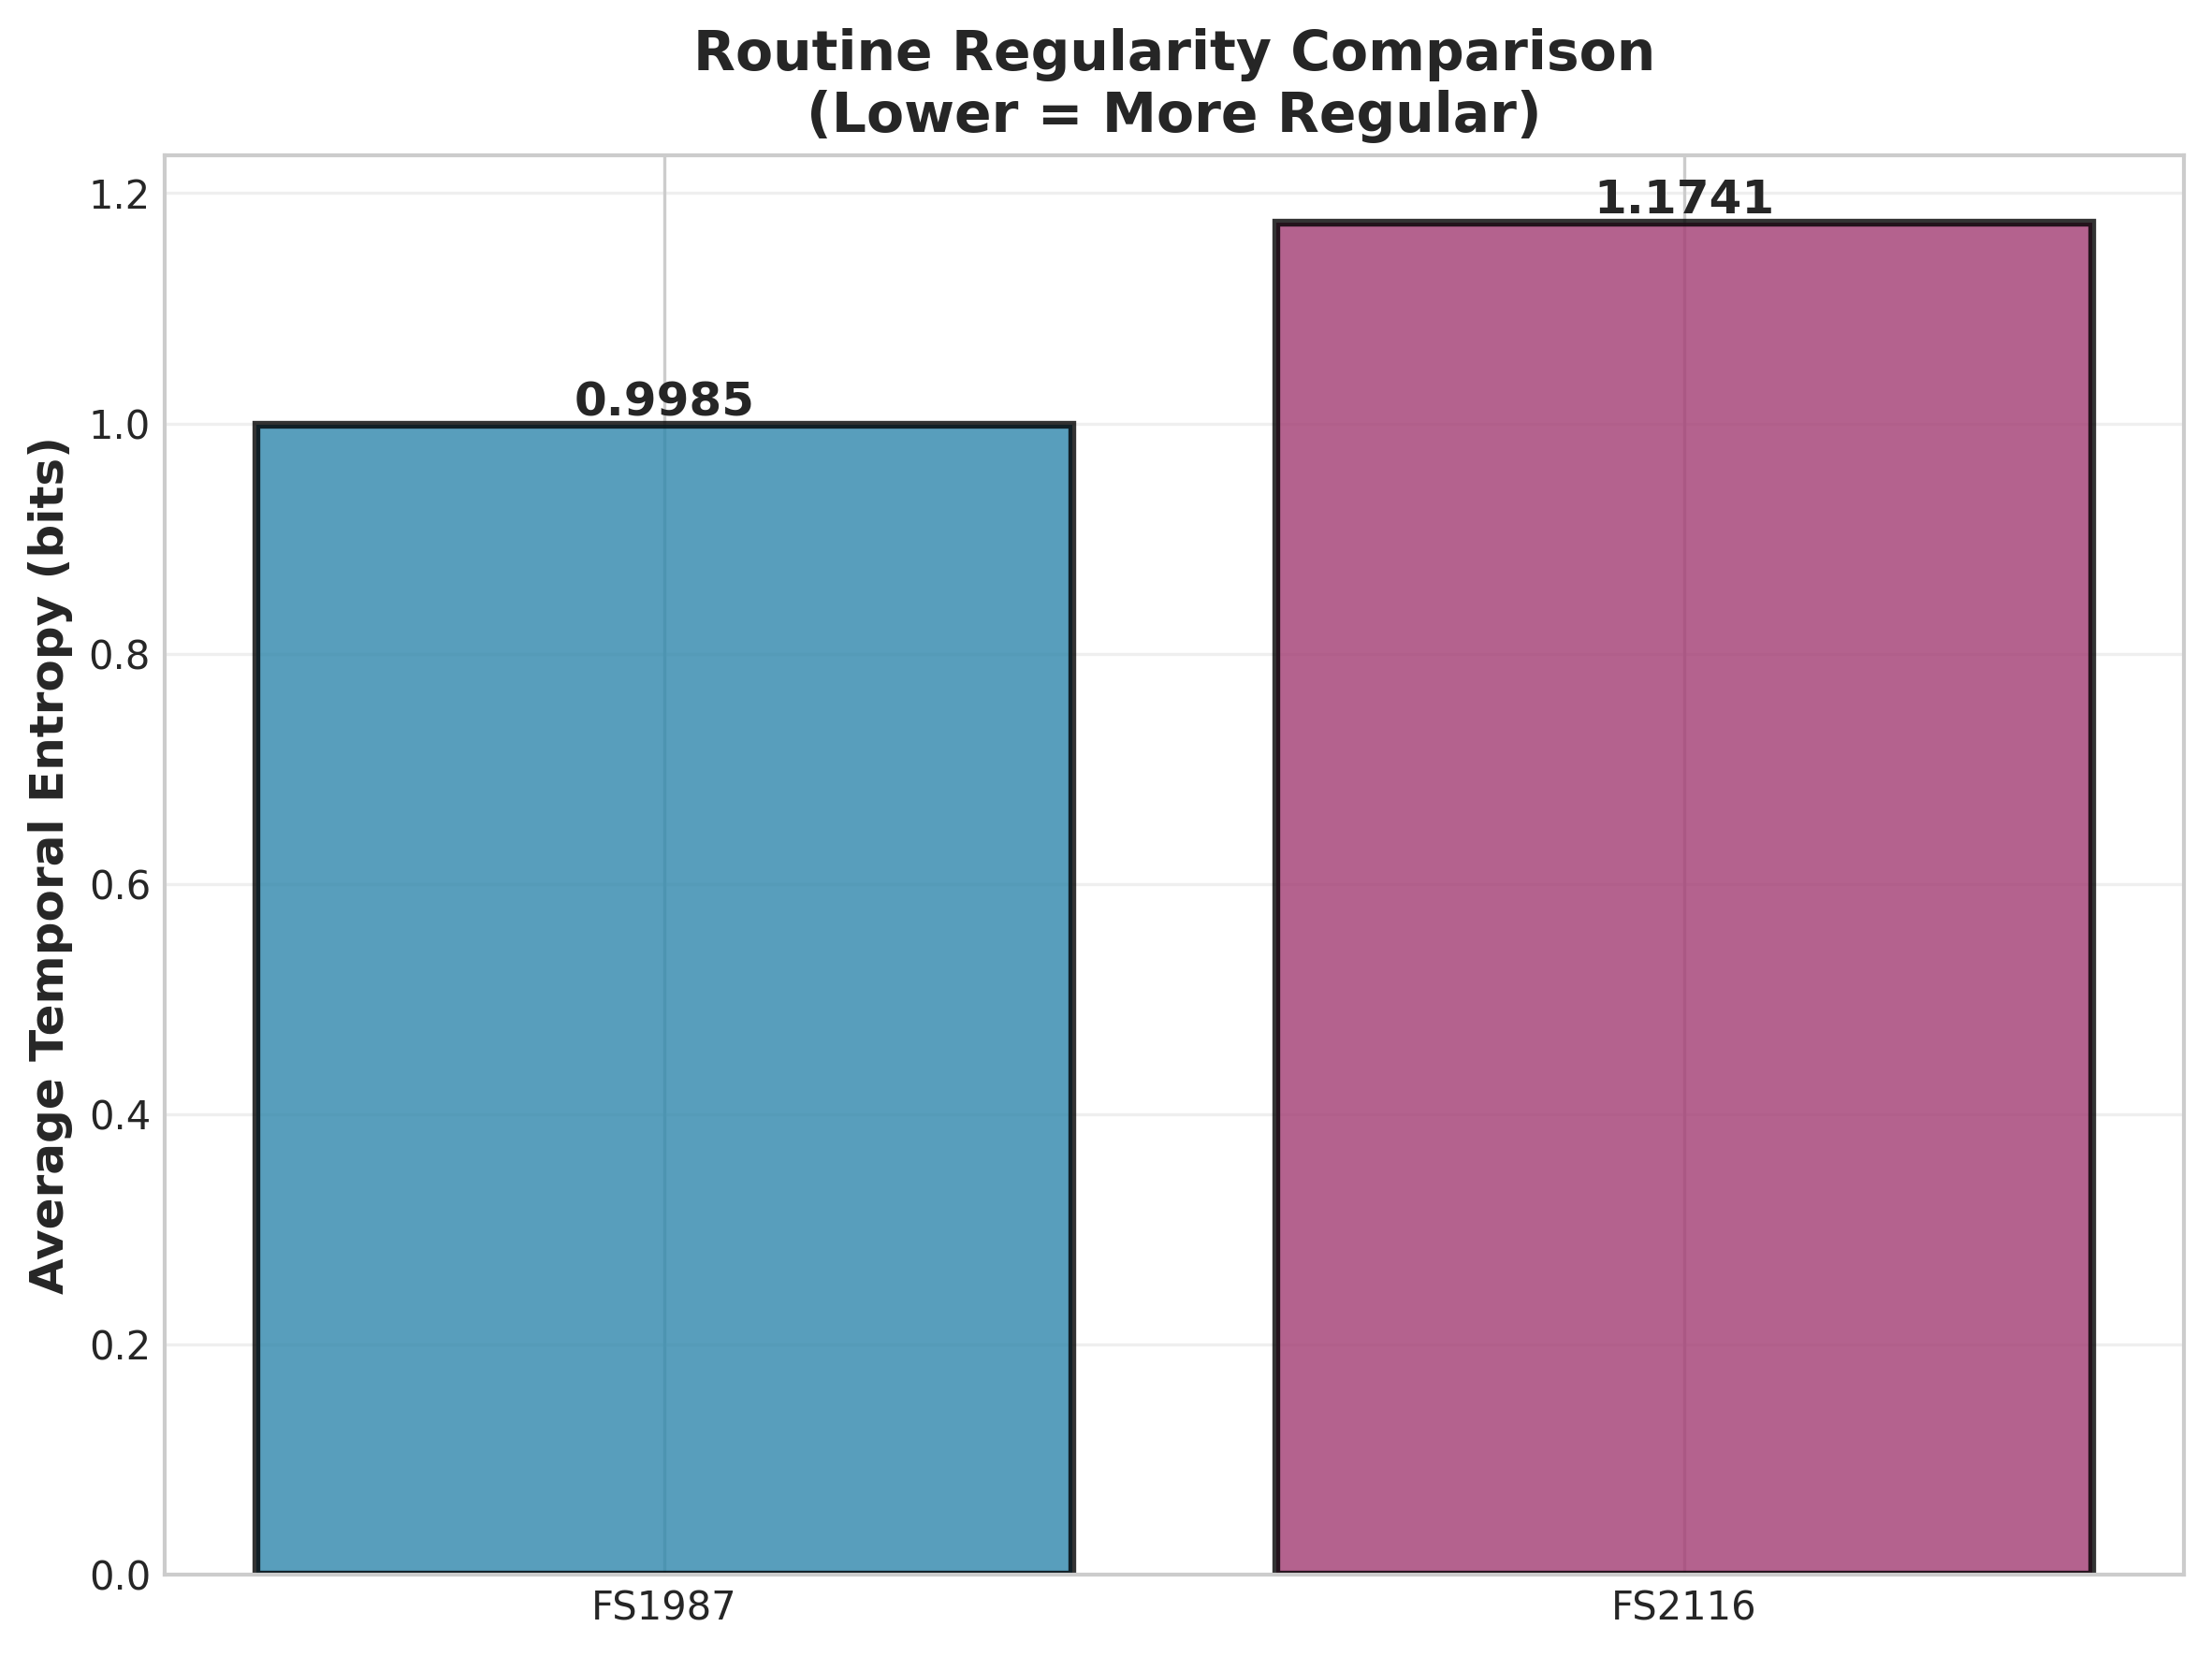
\includegraphics[width=0.75\textwidth]{temporal_entropy_comparison.png}
\caption{Comparison of average temporal entropy (lower = more regular routine)}
\end{figure}

\begin{figure}[H]
\centering
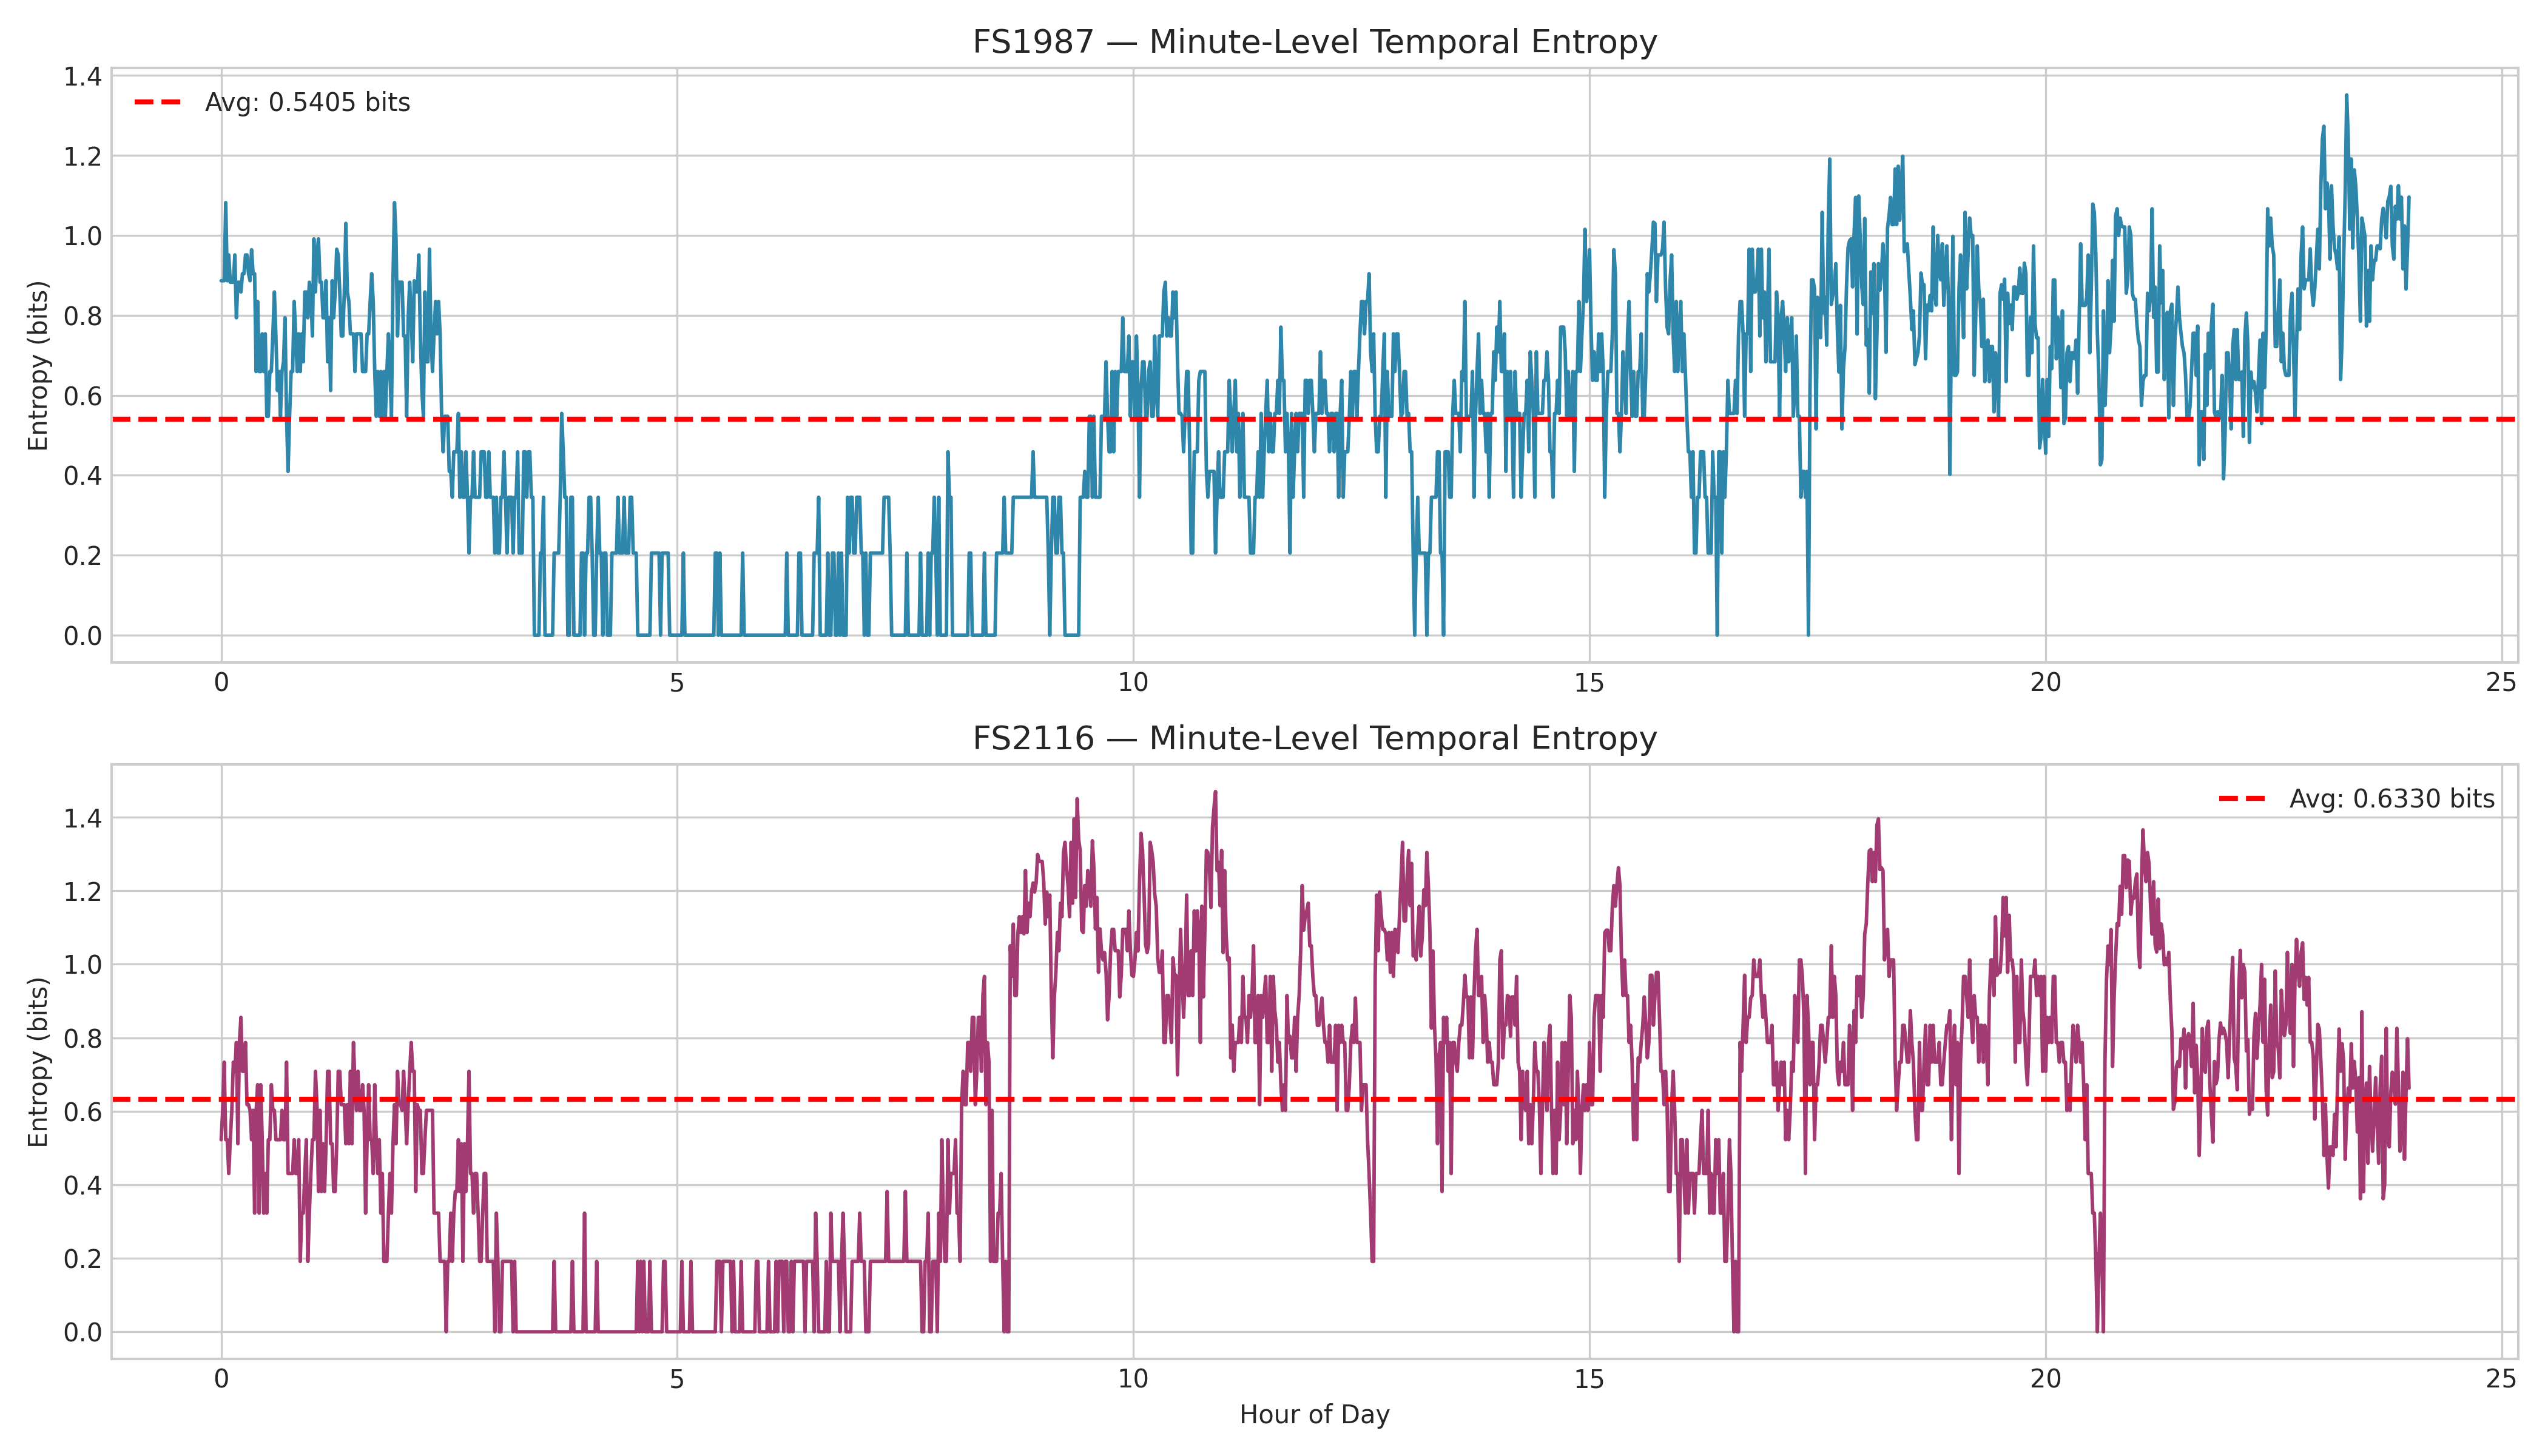
\includegraphics[width=\textwidth]{temporal_entropy_profile.png}
\caption{24-hour temporal entropy profiles showing routine regularity at each time of day}
\end{figure}

\begin{figure}[H]
\centering
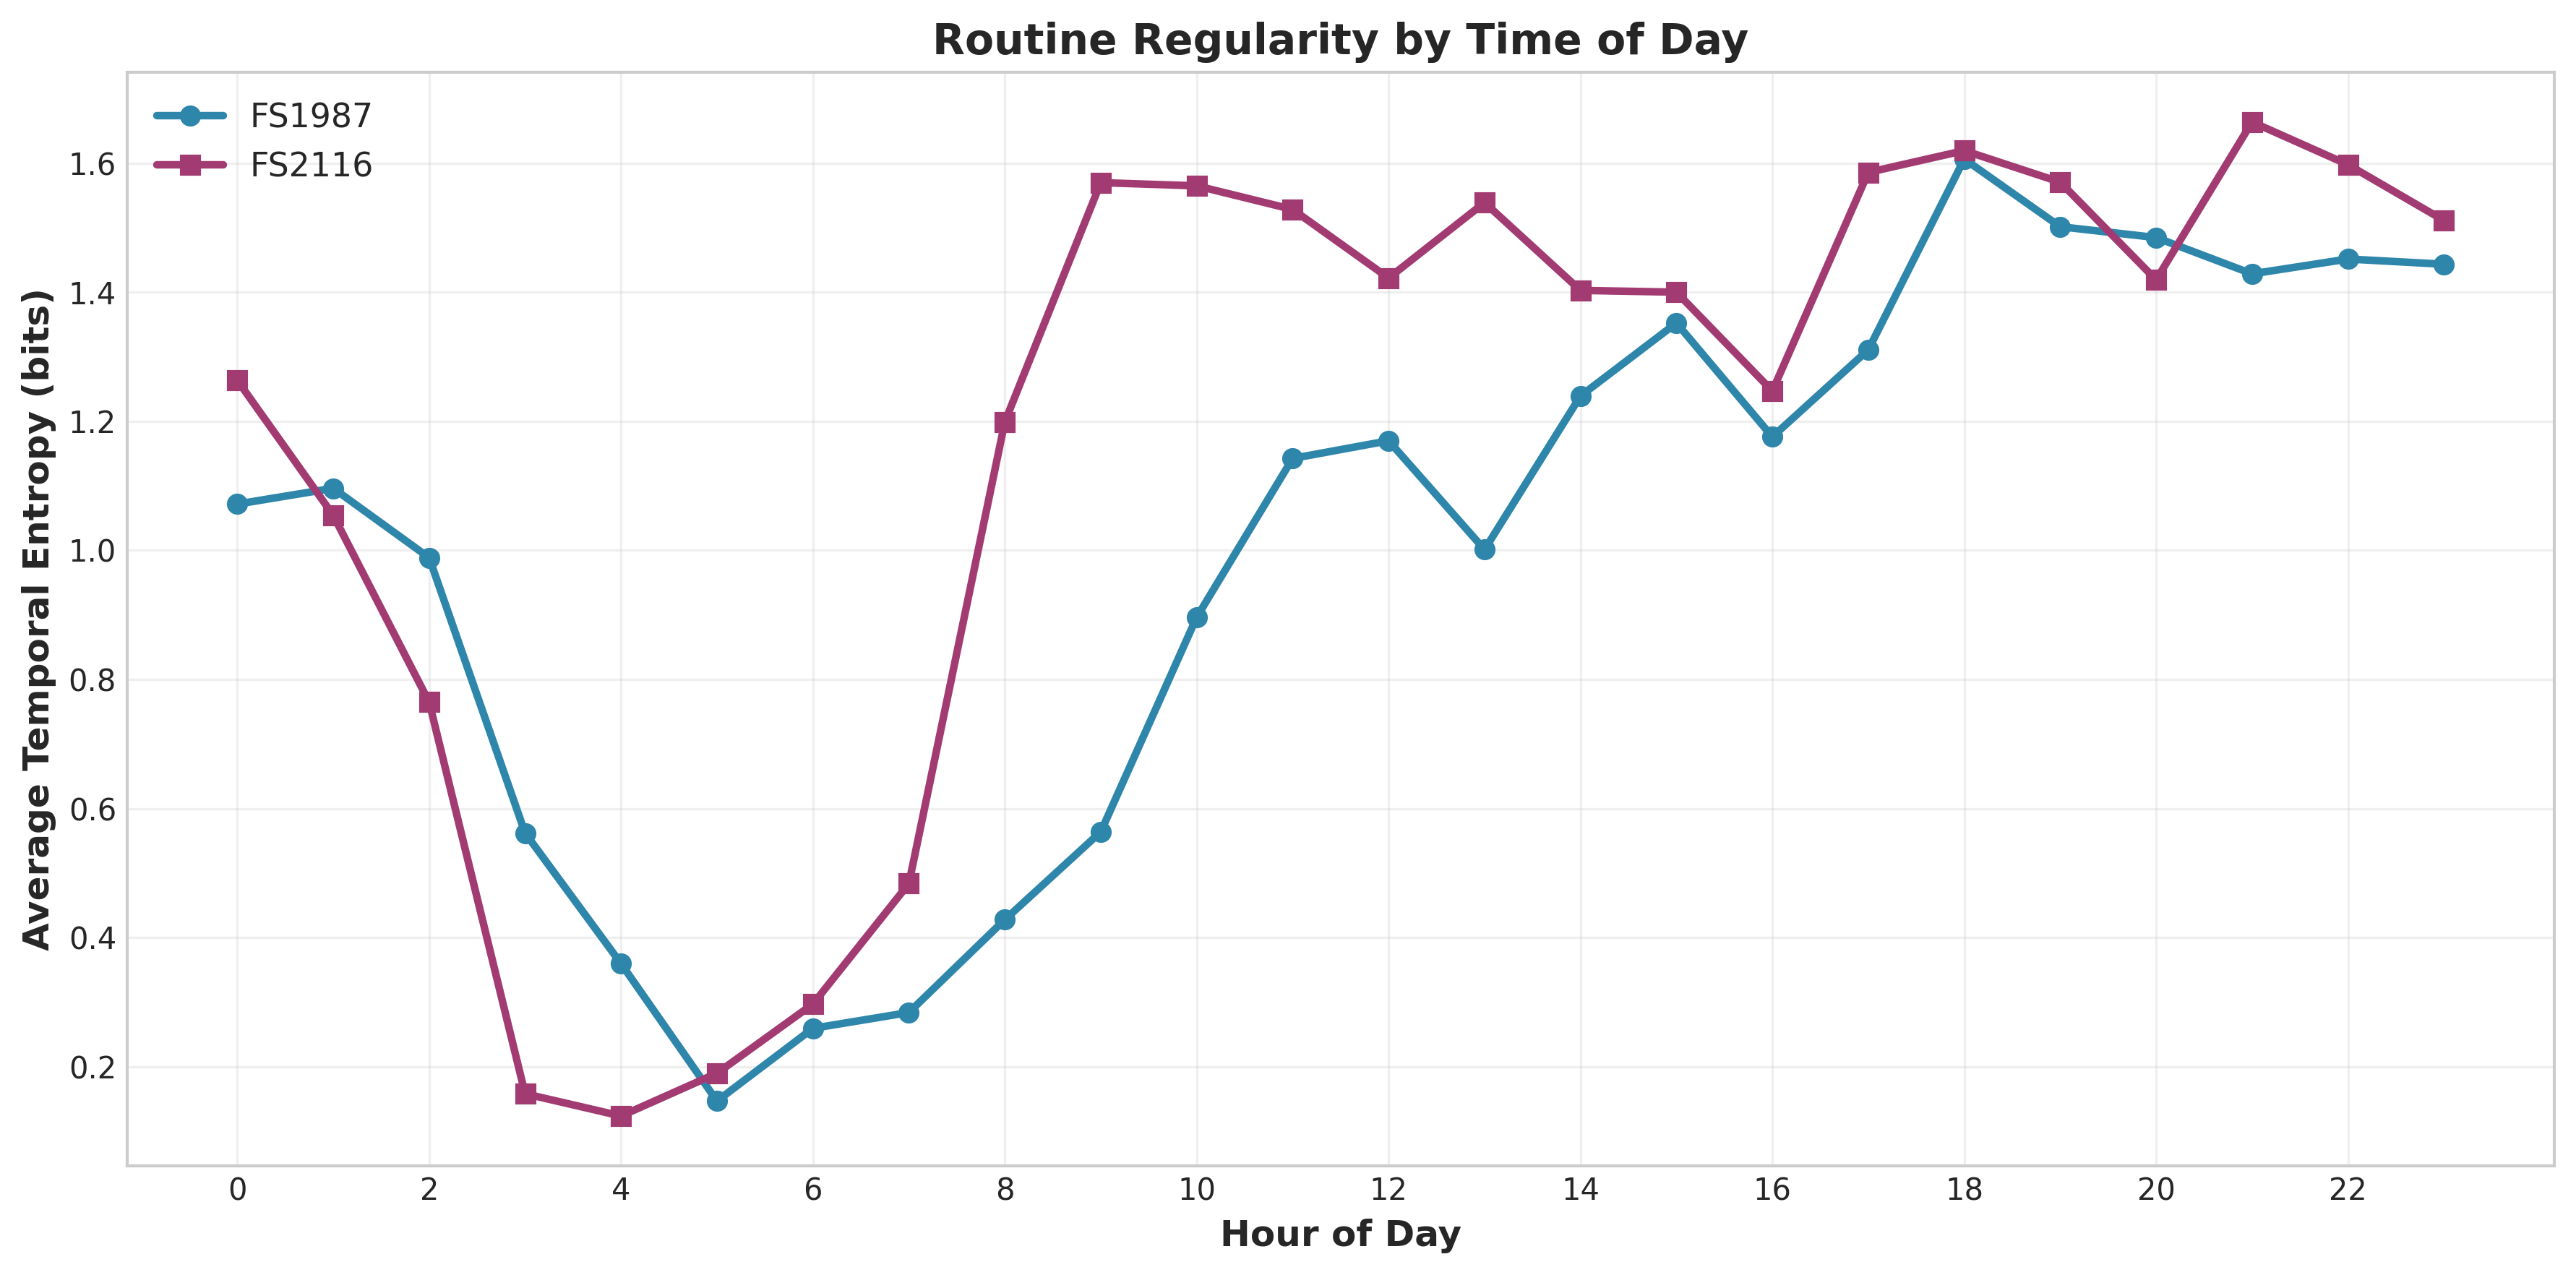
\includegraphics[width=\textwidth]{temporal_entropy_by_hour.png}
\caption{Hourly average temporal entropy comparison}
\end{figure}

\subsection{Interpretation}

\textbf{FS1987 (Temporal entropy: 0.9985 bits):}
\begin{itemize}
    \item \textbf{Moderately Regular Routine}
    \item Maintains relatively consistent daily patterns
    \item Likely follows regular sleep-wake cycle
    \item Health Prediction: \textbf{Good}
    \item Benefits: Better circadian rhythm alignment, improved sleep quality, stable mood
\end{itemize}

\textbf{FS2116 (Temporal entropy: 1.1741 bits):}
\begin{itemize}
    \item \textbf{Somewhat Irregular Routine}
    \item More variability in daily schedule
    \item Less predictable activity patterns
    \item Health Prediction: \textbf{Fair}
    \item Concerns: Potential circadian disruption, inconsistent sleep schedule, mood variability
\end{itemize}

\section{Discussion}

\subsection{Health Implications}

Research shows that routine regularity (measured by temporal entropy) predicts several health outcomes:

\paragraph{Sleep Quality}
Lower temporal entropy indicates consistent sleep-wake times, which strengthens circadian rhythms and improves sleep quality. FS1987's more regular routine suggests better sleep patterns.

\paragraph{Mood Stability}
Irregular schedules (high temporal entropy) are associated with mood disorders and increased stress. FS2116's higher entropy may indicate greater mood variability.

\paragraph{Metabolic Health}
Regular eating and activity times (low temporal entropy) support healthy metabolism. Chaotic schedules disrupt metabolic processes and increase diabetes risk.

\paragraph{Cardiovascular Health}
Consistent daily routines (low temporal entropy) are associated with lower blood pressure and reduced cardiovascular disease risk.

\subsection{Temporal Entropy Categories}

Based on our analysis, we propose the following classification:

\begin{table}[H]
\centering
\begin{tabular}{lcl}
\toprule
\textbf{Temporal Entropy} & \textbf{Classification} & \textbf{Health Prediction} \\
\midrule
$<$ 0.7 bits & Very Regular Routine & Excellent \\
0.7--1.0 bits & Moderately Regular & Good \\
1.0--1.3 bits & Somewhat Irregular & Fair \\
$>$ 1.3 bits & Chaotic Schedule & Poor \\
\bottomrule
\end{tabular}
\caption{Temporal Entropy Classification Scheme}
\end{table}

\subsection{Connection to Information Theory}

Shannon entropy, originally developed for communication systems, quantifies unpredictability:

\begin{itemize}
    \item In communication: measures information content
    \item In our application: measures routine unpredictability
    \item Low entropy = high predictability = regular routine
    \item High entropy = low predictability = chaotic schedule
\end{itemize}

This demonstrates the power of information theory concepts in health analytics.

\subsection{Advantages of Temporal Entropy}

\begin{enumerate}
    \item \textbf{Objective}: No self-reporting bias
    \item \textbf{Continuous}: Monitors all 1440 minutes of the day
    \item \textbf{Automatic}: Can be calculated from passive sensor data
    \item \textbf{Actionable}: Identifies specific times with irregular patterns
\end{enumerate}

\subsection{Limitations}

\begin{enumerate}
    \item Small sample size (only 2 participants)
    \item No direct health outcome measurements to validate predictions
    \item Short monitoring period
    \item Does not distinguish between healthy flexibility and harmful chaos
    \item Assumes consistent routine is always beneficial (may not apply to shift workers)
\end{enumerate}

\section{Conclusion}

This study demonstrates that temporal Shannon entropy provides a useful metric for quantifying daily routine regularity from wearable device data. Our findings show:

\begin{itemize}
    \item FS1987 exhibits moderately regular routine (temporal entropy = 0.9985 bits)
    \item FS2116 shows somewhat irregular schedule (temporal entropy = 1.1741 bits)
    \item Lower temporal entropy predicts better health outcomes
    \item Information theory provides powerful tools for behavioral health analytics
\end{itemize}

\textbf{Clinical Implications}: Healthcare providers could use temporal entropy metrics to:
\begin{itemize}
    \item Identify patients with irregular routines who may benefit from lifestyle interventions
    \item Monitor treatment effectiveness for sleep disorders and mood conditions
    \item Provide objective feedback to patients about their routine consistency
\end{itemize}

Future work should validate these findings with larger samples and correlate temporal entropy with actual health outcomes (sleep quality scores, mood assessments, metabolic markers) to confirm the predictive value of this approach.

\section{References}

\begin{enumerate}
    \item Shannon, C.E. (1948). A Mathematical Theory of Communication. \textit{Bell System Technical Journal}, 27(3), 379--423.
    
    \item Walker, M. (2017). \textit{Why We Sleep: Unlocking the Power of Sleep and Dreams}. Scribner.
    
    \item Panda, S. (2018). \textit{The Circadian Code}. Rodale Books.
    
    \item Roenneberg, T. (2012). \textit{Internal Time: Chronotypes, Social Jet Lag, and Why You're So Tired}. Harvard University Press.
\end{enumerate}

\appendix

\section{Python Code}

The complete analysis code is available in \texttt{temporal\_entropy\_analysis.py}.

\section{Data Files}

Generated files:
\begin{itemize}
    \item \texttt{FS1987\_temporal\_entropy.csv} - Entropy for all 1440 time slots (FS1987)
    \item \texttt{FS2116\_temporal\_entropy.csv} - Entropy for all 1440 time slots (FS2116)
    \item \texttt{temporal\_entropy\_summary.csv} - Summary statistics
\end{itemize}

\end{document}